\documentclass[12pt,a4paper]{article}
%\usepackage{ctex}
\usepackage{amsmath,amscd,amsbsy,amssymb,latexsym,url,bm,amsthm}
\usepackage{epsfig,graphicx,subfigure}
\usepackage{enumitem,balance}
\usepackage{wrapfig}
\usepackage{mathrsfs,euscript}
\usepackage[x11names,svgnames,dvipsnames]{xcolor}
\usepackage{hyperref}
\usepackage[vlined,ruled,commentsnumbered,linesnumbered]{algorithm2e}
\usepackage{listings}
\usepackage{multicol}


\usepackage{tikz}
\usepackage{verbatim}
\usepackage{preview}
% \PreviewEnvironment{tikzpicture}
% \usetikzlibrary{trees}

\usepackage{fontspec}
\renewcommand{\listalgorithmcfname}{List of Algorithms}
\renewcommand{\algorithmcfname}{Alg}

\newtheorem{theorem}{Theorem}
\newtheorem{lemma}[theorem]{Lemma}
\newtheorem{proposition}[theorem]{Proposition}
\newtheorem{corollary}[theorem]{Corollary}
\newtheorem{exercise}{Exercise}
\newtheorem*{solution}{Solution}
\newtheorem{definition}{Definition}
\theoremstyle{definition}


%\numberwithin{equation}{section}
%\numberwithin{figure}{section}

\renewcommand{\thefootnote}{\fnsymbol{footnote}}

\newcommand{\postscript}[2]
 {\setlength{\epsfxsize}{#2\hsize}
  \centerline{\epsfbox{#1}}}

\renewcommand{\baselinestretch}{1.0}

\setlength{\oddsidemargin}{-0.365in}
\setlength{\evensidemargin}{-0.365in}
\setlength{\topmargin}{-0.3in}
\setlength{\headheight}{0in}
\setlength{\headsep}{0in}
\setlength{\textheight}{10.1in}
\setlength{\textwidth}{7in}
\makeatletter \renewenvironment{proof}[1][Proof] {\par\pushQED{\qed}\normalfont\topsep6\p@\@plus6\p@\relax\trivlist\item[\hskip\labelsep\bfseries#1\@addpunct{.}]\ignorespaces}{\popQED\endtrivlist\@endpefalse} \makeatother
\makeatletter
\renewenvironment{solution}[1][Solution] {\par\pushQED{\qed}\normalfont\topsep6\p@\@plus6\p@\relax\trivlist\item[\hskip\labelsep\bfseries#1\@addpunct{.}]\ignorespaces}{\popQED\endtrivlist\@endpefalse} \makeatother


\definecolor{codegreen}{rgb}{0.44,0.68,0.28}
\definecolor{codegray}{rgb}{0.5,0.5,0.5}
\definecolor{codepurple}{rgb}{0.58,0,0.82}
\definecolor{backcolour}{rgb}{0.96,0.96,0.96}

\lstset{
language=C++,
frame=shadowbox,
keywordstyle = \color{blue}\bfseries,
commentstyle=\color{codegreen},
tabsize = 4,
backgroundcolor=\color{backcolour},
numbers=left,
numbersep=5pt,
breaklines=true,
emph = {int,float,double,char},emphstyle=\color{orange},
emph ={[2]const, typedef},emphstyle = {[2]\color{red}} }



\begin{document}
\noindent

%========================================================================
\noindent\framebox[\linewidth]{\shortstack[c]{
\Large{\textbf{Lab07-Trees}}\vspace{1mm}\\
VE281 - Data Structures and Algorithms, Xiaofeng Gao, TA: Qingmin Liu, Autumn 2019}}
%CS26019 - Algorithm Design and Analysis, Xiaofeng Gao, Autumn 2019}}
\begin{center}
\footnotesize{\color{red}$*$ Please upload your assignment to website. Contact webmaster for any questions.}

\footnotesize{\color{blue}$*$ Name:Wu Jiayao  \quad Student ID:517370910257 \quad Email: jiayaowu1999@sjtu.edu.cn}
\end{center}

{\color{blue}\textbf{Hint:} You can use the package \textbf{tikz} to draw trees.}

\begin{figure}[h]
\centering
\begin{tikzpicture}
	[thick,scale=0.8, every node/.style={scale=1.2}]
	\node {root}
	child {node {1}
		child {node {2}
			child {node {3}}
		}
		child [missing] {}
		child {node {3}
			child {node {2}}
		}
	}	
  	child [missing] {}	
	child [missing] {}
	child [missing] {}	
	child [missing] {}	
	child { node {2}
		child {node {1}
			child {node {3}}
		}
		child [missing] {}
		child {node {3}
			child {node {1}}
		}
	}	
	child [missing] {}	
	child [missing] {}
	child [missing] {}	
	child [missing] {}	
	child { node {3}
		child {node {1}
			child {node {2}}
		}
		child [missing] {}
		child {node {2}
			child {node {1}}
		}
	};
	\end{tikzpicture}
	\end{figure}

\begin{enumerate}

\item	Red-black Tree
	\begin{enumerate}
		\item Suppose that we insert a sequence of keys 9, 3, 1 into an initially empty red-black tree. Draw the resulting red-black tree.
		
		\item Suppose that we further insert key 6 into the red-black tree you get in Problem (1-a). Draw the resulting red-black tree.
		
		\item Suppose that we further insert keys 2, 8 into the red-black tree you get in Problem (1-b). Draw the resulting red-black tree.
		
		\item Suppose that we further insert key 7 into the red-black tree you get in Problem (1-c). Draw the resulting red-black tree.
		
		\item Suppose that we further insert keys 4, 5 into the red-black tree you get in Problem (1-d). Draw the resulting red-black tree.
		
	\end{enumerate}
	
	When you draw the red-black tree, please indicate the color of each node in the tree.
For example, you can color each node or put a letter \textbf{b/r} near each node.

\begin{solution} 
\begin{enumerate}
    \item  $\ $
    \begin{figure}[h]
        \centering
        \begin{tikzpicture}
            \node{3b}
            child{node{1r}}
            child{node{9r}};
        \end{tikzpicture}
    \end{figure}
\newpage
    \item $\ $
    \begin{figure}[h]
        \centering
        \begin{tikzpicture}
            \node{3b}
            child{node{1b}}
            child{node{9b}
                child{node{6r}}
                child[missing]{}
            };
        \end{tikzpicture}
    \end{figure}
    \item $\ $
    \begin{figure}[h]
        \centering
        \begin{tikzpicture}
            \node{3b}
            child{node{1b}
                child[missing]{}
                child{node{2r}}
            }
            child[missing]{}
            child{node{8b}
                child{node{6r}}
                child{node{9r}}
            };
        \end{tikzpicture}
    \end{figure}
    \item $\ $
    \begin{figure}[h]
        \centering
        \begin{tikzpicture}
            \node{3b}
            child{node{1b}
                child[missing]{}
                child{node{2r}}
            }
            child[missing]{}
            child{node{8r}
                child{node{6b}
                    child[missing]{}
                    child{node{7r}}}
                child{node{9b}}
            };
        \end{tikzpicture}
    \end{figure}
\newpage
    \item $\ $
    \begin{figure}[h]
        \centering
        \begin{tikzpicture}
            \node{6b}
            child{node{3r}
                child{node{1b}
                    child[missing]{}
                    child{node{2r}}
                    }
                child{node{4b}
                    child[missing]{}
                    child{node{5r}}
                    }
            }
            child[missing]{}
            child{node{8r}
                child{node{7b}}
                child{node{9b}}};
        \end{tikzpicture}
    \end{figure}
\end{enumerate}
\end{solution}

\item  Show the alphabet trie for the following collection of words: \{chicken, goose, deer, horse, antelope, anteater, goldfish, ant, goat, duck\}.

\begin{solution} 
\begin{figure}[h]
    \centering
    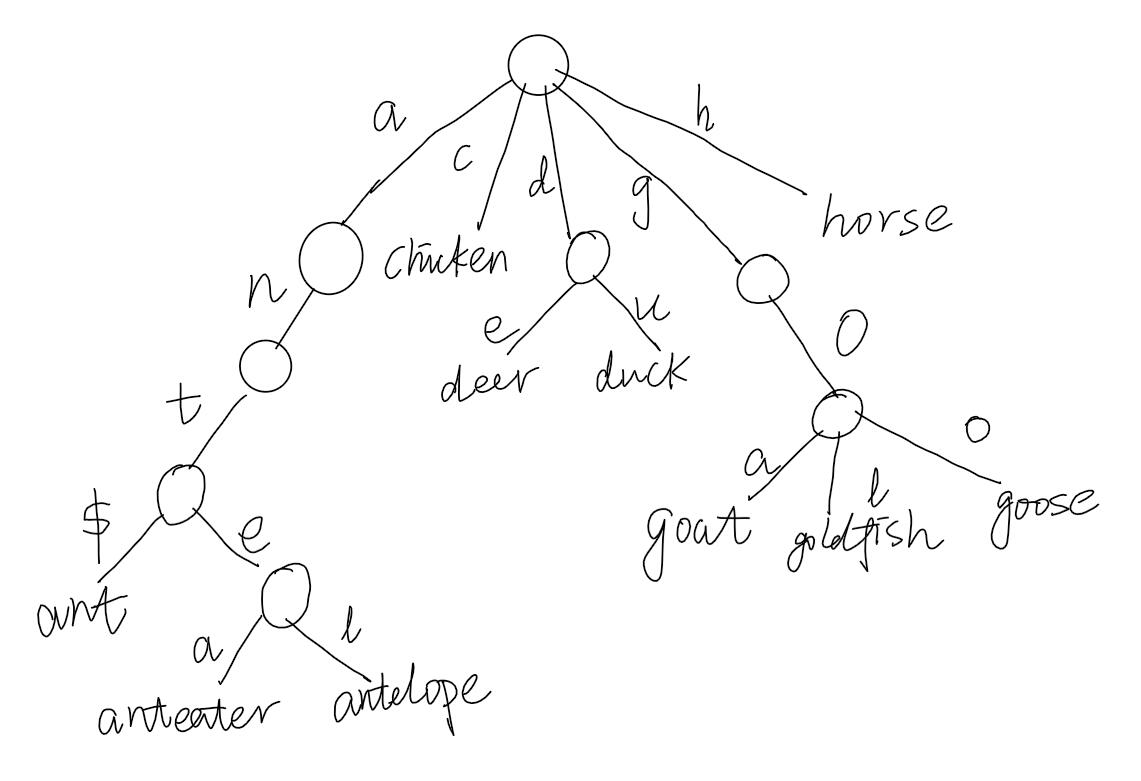
\includegraphics[width=0.7\textwidth]{1.jpg}
    \caption{Handmade tries}
    \label{tries}
\end{figure}
\end{solution}

\newpage
\item  Show that any arbitrary n-node binary search tree can be transformed into any other arbitrary n-node binary search tree using $O(n)$ rotations. 

	{\color{blue} Hint: First show that at most $n − 1$ right rotations suffice to transform the tree into a right-skewed binary
search tree.}

\begin{solution} 

    \par For every node that is at the left of the root, if it has a right child, rotate left (the old left child becomes the root, the old root becomes its left child). For every node that is at the right of the root, if it has a left child, rotate right (the old right child becomes the root, the old root becomes its right child). Such operations is $\mathcal{O}(n)$, since it visits every node once. The result tree (just call it a tree) is an increasing, going from left to right chain, with one node marked as root.
    \par Such operations above can be reversed to form another binary search tree from an increasing, going from left to right chain. Hence, we do a set of above operations to turn a BST into a chain, then change the root of the chain, do the reverse operations, then we get a new BST tree. It takes $\mathcal{O}(n)$ operations. 
\end{solution}

\item  Suppose that an AVL tree insertion breaks the AVL balance condition. Suppose node $P$ is the first node that has a balance condition violation in the insertion access path from the leaf. Assume the key is inserted into the left subtree of $P$ and the left child of $P$ is node $A$. Prove the following claims:
	\begin{enumerate}
		\item  Before insertion, the balance factor of node $P$ is 1. After insertion and before applying rotation to fix the violation, the balance factor of node $P$ is 2.
		\item Before insertion, the balance factor of node $A$ is 0. After insertion and before applying rotation to fix the violation, the balance factor of node $A$ cannot be 0.
	\end{enumerate}
	
\begin{solution} 
\begin{enumerate}
    \item The problem can be transformed into solving an equation, since insertion is done on the left subtree. By insertion $h_l \leq h_l^{'} \leq h_l+1$.
    \begin{equation}
        \left\{
                \begin{array}{lr}
                     |B_P| = |h_l-h_r| \leq 1  \\
                     |B_P^{'}| = |h_l^{'}-h_r| > 1  \\ 
                \end{array}
        \right.
    \end{equation}
    If $h_l^{'}=h_l$, there is no solution, thus no balance is broken. Hence, $h_l^{'}=h_l+1$, that $h_l-h_r$=1, which means that the factor of node P is 1. After insertion and before fixing, the factor of node P is 2.
    \item The problem can be transformed into solving an equation, since insertion is done on the left subtree. By insertion $h_l \leq h_l^{'} \leq h_l+1$.
    \begin{equation}
        \left\{
                \begin{array}{lr}
                     |B_P| = |h_l-h_r| \leq 1  \\
                     |B_P^{'}| = |h_l^{'}-h_r| > 1  \\ 
                \end{array}
        \right.
    \end{equation}
    If $h_l^{'}=h_l$, there is no solution, thus no balance is broken. Hence, $h_l^{'}=h_l+1$, $h_l-h_r$=1.
    Denote the left child of A is M, the right is N. What about $h_M$ and $h_N$?
    \begin{itemize}
        \item $h_M=h_N+1$. If the insertion happens in subtree N, no balance is broken. If happens in subtree M, the first node will be A rather than P, since $B_A$ will be 2.
        \item $h_N=h_M+1$. If the insertion happens in subtree M, no balance is broken. If happens in subtree N, the first node will be A rather than P, since $B_A$ will be -2.
        \item $h_N=h_M$. It is correct. When inserted at rather M or N, $h_l^{'}=h_l+1$, $|B_A|>0$. Since $h_l^{'}-h_r$=2, balance is broken first at P.
    \end{itemize}
    Hence ,$h_N=h_M$, the balance factor of A is 0. After insertion, the balance factor of node A cannot be 0.
\end{enumerate}
\end{solution}

\end{enumerate}

%========================================================================
\end{document}